\documentclass{article}

% if you need to pass options to natbib, use, e.g.:
% ©PassOptionsToPackage{numbers, compress}{natbib}
% before loading nips_2016
%
% to avoid loading the natbib package, add option nonatbib:
% \usepackage[nonatbib]{nips_2016}

\usepackage[final]{nips_2016}

% to compile a camera-ready version, add the [final] option, e.g.:
% \usepackage[final]{nips_2016}

\usepackage[utf8]{inputenc} % allow utf-8 input
\usepackage[T1]{fontenc}    % use 8-bit T1 fonts
\usepackage{hyperref}       % hyperlinks
\usepackage{url}            % simple URL typesetting
\usepackage{booktabs}       % professional-quality tables
\usepackage{amsfonts}       % blackboard math symbols
\usepackage{amssymb}
\usepackage{amsmath}
\usepackage{bbm}
\usepackage{nicefrac}       % compact symbols for 1/2, etc.
\usepackage{microtype}      % microtypography
\usepackage{caption}
\usepackage{float}
\usepackage{graphicx}
\usepackage{subfig}
\usepackage{wrapfig}
\usepackage{authblk}

\graphicspath{ {./} }

\title{A multi-modal neural network for learning cis and trans regulation of stress response in S. cerevisiae}

% The \author macro works with any number of authors. There are two
% commands used to separate the names and addresses of multiple
% authors: \And and \AND.
%
% Using \And between authors leaves it to LaTeX to determine where to
% break the lines. Using \AND forces a line break at that point. So,
% if LaTeX puts 3 of 4 authors names on the first line, and the last
% on the second line, try using \AND instead of \And before the third
% author name.

\author[1,2,3]{Boxiang Liu}
\author[4]{Nadine Hussami}
\author[3,5]{Avanti Shrikumar}
\author[3]{Tyler Shimko}
\author[6]{Salil Bhate}
\author[6]{Scott Longwell}
\author[2,3]{Stephen Montgomery}
\author[3,6]{Anshul Kundaje}
\affil[ ]{$^1$Departments of Biology, $^2$Pathology, $^3$Genetics, $^4$Statistics, $^5$Computer Science, and $^6$Bioengineering, Stanford University}
\affil[ ]{\textit{\{bliu2,nadinehu,avanti,tshimko,bhate,longwell,smontgom,akundaje\}@stanford.edu}}

\begin{document}

\maketitle

\begin{abstract}

Understanding gene regulatory mechanisms is a central problem in computational biology. Here, we explore the use of interpretable multi-modal neural networks to learn cis and trans regulation of stress response in the budding yeast \textit{Saccharomyces cerevisiae}. We formulate the problem as a regression task, where the goal is learn a model that can accurately predict the real-valued gene expression of all genes across 173 different stress conditions based on two complementary regulatory inputs - a cis component represented by the raw promoter sequence of each gene and a trans component represented by the real-valued expression of a subset of regulatory genes (transcription factors and signaling molecules). The multimodal neural network includes a convolutional module to learn predictive patterns from the raw promoter sequences, a dense module to derive features from regulator expression and an integration module that learns cis-trans interactions. We use a variety of cross-validation settings to evaluate the performance of the model (held-out genes, held-out stress conditions). In all cases, the models achieve high performance and substantially outperform other state-of-the-art methods such as boosting algorithms that pre-defined cis-regulatory features (known motifs). We then use an efficient backpropagation algorithm that we recently developed to interpret the model. We interpret the model to reveal dynamic promoter sequence motif grammars, trans regulator modules and motif-regulator associations affecting individual genes and gene modules in diverse stress conditions. Our model correctly identifies known master regulators such as MSN4/MSN2, USV1, YVH1 as well as several stress-specific factors. We also use our models to perform in silico knock-out/knock-in experiments. In a MSN2/4 knockout experiment, we demonstrate that in silico predictions of target gene changes strongly correlate with the results of the corresponding knockout microarray experiment.
  
\end{abstract}

\section{Introduction}

The faithful prediction of gene expression levels based on primary DNA sequence is a critical milestone toward fully comprehending cellular dynamics. Modulation of expression levels allows the host cell to react and adapt to its environment, enhancing the ability of the cell to survive in the face of constantly-evolving pressures. Many factors have the ability to influence gene expression levels including environmental stresses, the cell cycle, and stochastic fluctuations of cellular states. The cell can perceive these changes using molecular sensors, which further transmit information through molecular signaling cascades, ultimately resulting in activation of transcriptional regulatory elements. These regulatory elements have the capacity to bind genomic DNA in a specific manner and activate or repress expression of genes to control the cell's response to the sensed change in state.

Expression levels can, therefore, be conceptualized at the most basic level as the output of a complex function of regulatory element/DNA interactions. Specifically, transcription factors, proteins that bind DNA and have the ability to activate or repress transcription of downstream genes, tend to preferentially bind certain DNA sequences termed “motifs.” However, expression of the downstream gene relies on both the presence of these motifs in the gene’s promoter sequence as well as the expression levels of the regulatory elements themselves. Without expression of the required regulatory element, the presence of the desired motif will fail to impact expression levels. Additionally, transcription factors exhibit what is known as "combinatorial control" over gene expression levels. In this scenario, the role of the transcription factor to either promote or repress gene expression is dictated by the presence of other transcription factors binding in the promoter region alongside it.

The budding yeast \textit{Saccharomyces cerevisiae} represents an ideal model organism to learn the grammar of regulatory element/promoter interactions. The transcriptional regulatory architecture of this yeast species is relatively simple, with the expression of the majority of genes being governed primarily by interactions between regulatory elements and the promoter sequence directly upstream of the gene. There exist very few long range genomic interactions in \textit{S. cerevisiae} such as those that would complicate such a project in higher-order organisms. We also expect relatively few binding interactions to have large effects on downstream transcription, as previous work has shown the overwhelming majority of promoters to be bound by fewer than 5 regulatory elements.

Here, we present a DNN architecture that is capable of predicting gene expression levels given the expression level of the complete set of \textit{S. cerevisiae} regulatory elements as well as the 1 kilobase sequence directly upstream of the transcription start site. This model takes advantage not only of count and spatial relationships between sequence motifs in the promoters of the individual genes, but also the amount of each regulatory element available to interact with those motifs. We demonstrate that our model achieves higher accuracy than the state-of-the-art method. Furthermore, since the sequence specificities of most DNA-binding regulatory elements have been experimentally validated \cite{deBoer:2011ic}, we show that our model provides sensible prediction based on existing knowledge about \textit{S. cerevisiae}.


\section{Methodology}

\subsection{Sequence module}
We treat one-hot encoded promoter sequences as black-and-white images of size $\{0,1\}^{4 \times 1000}$. The promoter sequences contain information about transcription factor binding motifs, each representing a consensus sequence (e.g. 'TGATCA'). Like an object in natural images, a motif appears in multiple promoter sequences and a given promoter can contain several instances of the same motif with slight variations. We use a 2-layer convolutional neural networks to detect such motifs. Mathematically, the 2D convolution layers with ReLU activation can be written as: 

\begin{equation} \label{eq1}
x_{ij}=\max \{ 0, \sum_{a=1}^{4} \sum_{b=1}^{l} W_{abj}^{seq} s_{(a)(i+b)} + b^{seq}\}
\end{equation} 

Where $s$ represents sequence input, $W^{seq}$ represents the weight for convolutional filters, $i$ represents the genomic location, $j$ represents filter number, $b^{seq}$ represents the bias, and $l$ represents the filter length. We use $l=9$ and $J=50$ filters for both convolutional layers with a subsampling rate of 1. To keep model prediction invariant to small motif shifts along the genomic axis, we apply 1D maxpooling with a subsampling rate of 4 after each convolutional layer. We applied batch normalization before each ReLU activation to mitigate covariate shifts during training and to accelerate learning. Since both strands of DNA encode identical information, we incorporated the reverse complement sequences into our model, effectively doubling the number of training examples, and used filter pairs with mirroring weights to detect each motif \cite{Anonymous:_KTX_iBy}. We used a fully connected layer with 512 units to integrate information across filters. 


\subsection{Regulator module}
Transcription factors and signaling molecules interact with each other through bi-, tri-molecular and even higher order reactions with no genomic-spatial constraint. We model the regulator input with a fully connected layer of 512 hidden units. Mathematically, 

\begin{equation} \label{eq2}
y=\max \{0, W^{reg}r + b^{reg}\}
\end{equation}

\subsection{Integration module}
In principle, the output from sequence module represents gene-specific information, and that from the regulator module represents condition-specific information. Treated separately, neither module will be able to predict the gene-condition interactions critical for accurate final prediction. We integrate two separate sources of information through a simple concatenation layer, and use a 2-layer fully connected network to model the interaction between motifs and regulators. 

\subsection{Dataset and Pre-processing}

We utilized the Gasch \cite{Gasch:2000wl} dataset which used microarray to measure a total of 6100 genes under 173 experimental conditions. The measurements were given as $log_2$ expression values representing the fold change w.r.t. the untreated reference condition. We used 1kbp sequences upstream of the transcription start site as the sequence predictors and a set of 472 transcription factors and signaling molecules as the regulator predictors. We used a 80-10-10 split among training, validation, and test datasets.


\subsection{Training methodology}
We trained our models using SGD with a learning rate of 0.01 and momentum of 0.5. We decrease the learning rates by half every five epoch if no improvement in validation accuracy is observed. All training were performed on Nvidia GeForce GTX 970 using Keras 1.2.2 with Tensorflow backend.


\section{Results}

\subsection{Regression and Classification Performances}
We compared our model against two previous models, GeneClass \cite{Middendorf:2004gta} and BDTree \cite{Ruan:2006hl}, using the same dataset by Gasch et al \cite{Gasch:2000wl}. The GeneClass model is a boosted alternating decision tree, and the BDTree model is a bidirectional regression tree. We trained our model to predict real-valued expression levels as well as discrete labels in $\{-1,0,1\}$ to represent upregulation, baseline, and downregulation. In the classification task, the dataset is discretized such that expression values in $[-\infty,-0.5]$ are converted to -1, $[-0.5,0.5]$ to 0, and $[0.5,\infty]$ to +1. Our best model outperformed the previous state-of-the-art by 16.6\% (Table \ref{table:classification performance}). In addition, our model achieved a pearson correlation of 0.82 for the regression task on the test set (Figure \ref{fig:correlation}). We were not able to compare our model with GeneClass or BDTree because the authors only reported classification results.

\begin{table}[!hbt]
\caption{Classification performance}
\centering
 \begin{tabular}{|c | c|} 
 \hline
 Method & Accuracy \\
 \hline
 GeneClass & 60.9\% \\ 
 \hline
 BDTree & 62.9\% \\
 \hline
 DNN & \textbf{79.5\%} \\
 \hline
\end{tabular}
\quad
\centering
 \begin{tabular}{|c | c c c|} 
 \hline
 {} & \multicolumn{3}{|l|}{Predicted by DNN} \\
  & Down & Baseline & Up \\ 
 \hline
 Down & 10.14 & 7.47 & 0.13 \\
 \hline
 Baseline & 3.29 & 59.77 & 3.02 \\
 \hline
 Up & 0.18 & 6.42 & 9.59 \\
 \hline
\end{tabular}
\label{table:classification performance}
\end{table}

\subsection{Recovering Known Motifs}
Existing models such as GeneClass and BDTree relies on existing motif annotations and lacks the ability to infer \textit{de novo} motif. Convolutional neural networks has the ability to learn filter weights and extracts motif information automatically. Studies have shown that known motifs can be recovered by CNNs trained on ChIP-seq data \cite{Quang:2016jt,Kelley:2016bv,Alipanahi:2015fb}. We found that our model learns both known and \textit{de novo} motifs. Figure 1 shows four known motifs recovered by our model. 


\begin{figure}
\centering
\subfloat[Correlation]{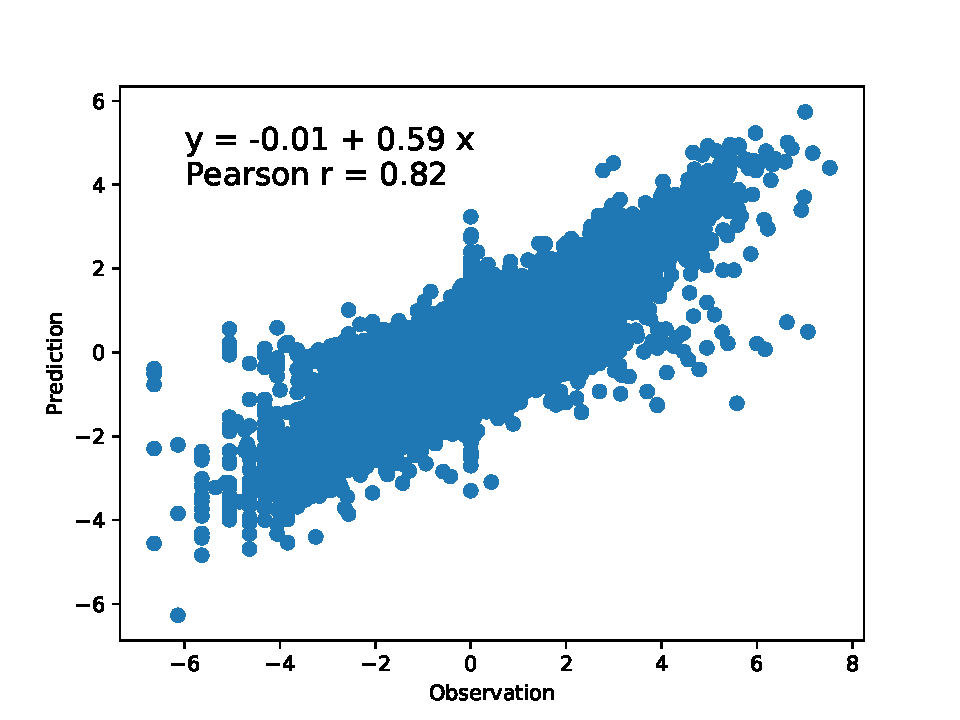
\includegraphics[trim={0.3in 0 0 0},clip,width=0.45\textwidth]{fig/correlation_tensor_product.pdf}\label{fig:correlation}}

\subfloat[DOT6P]{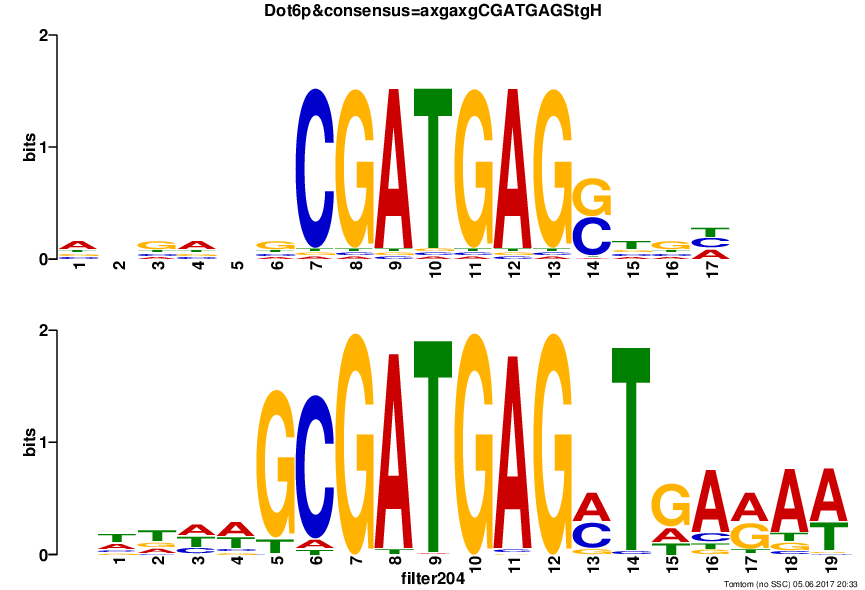
\includegraphics[width=0.2\textwidth]{fig/tomtom/dot6p_2.png}\label{fig:2a}}
\subfloat[RPN4P]{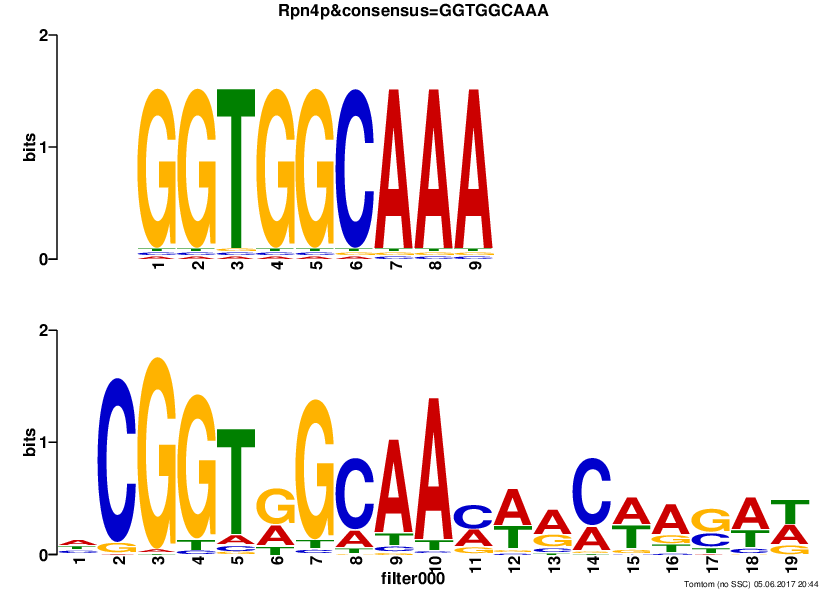
\includegraphics[width=.2\textwidth]{fig/tomtom/rpn4p.png}\label{fig:2b}}
\subfloat[SFP1P]{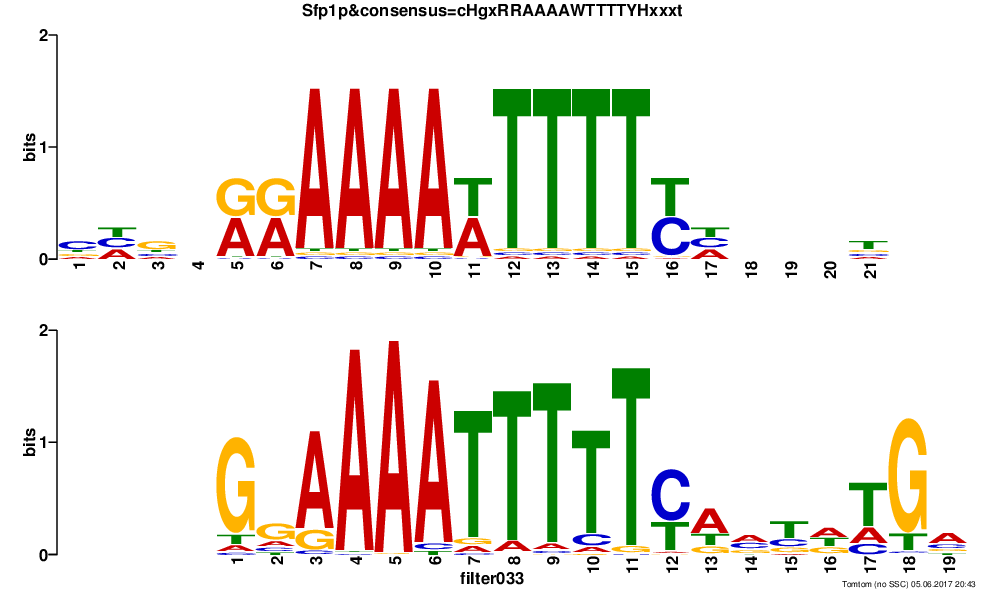
\includegraphics[width=.2\textwidth]{fig/tomtom/sfp1p_2.png}\label{fig:2c}}
\subfloat[STB3P]{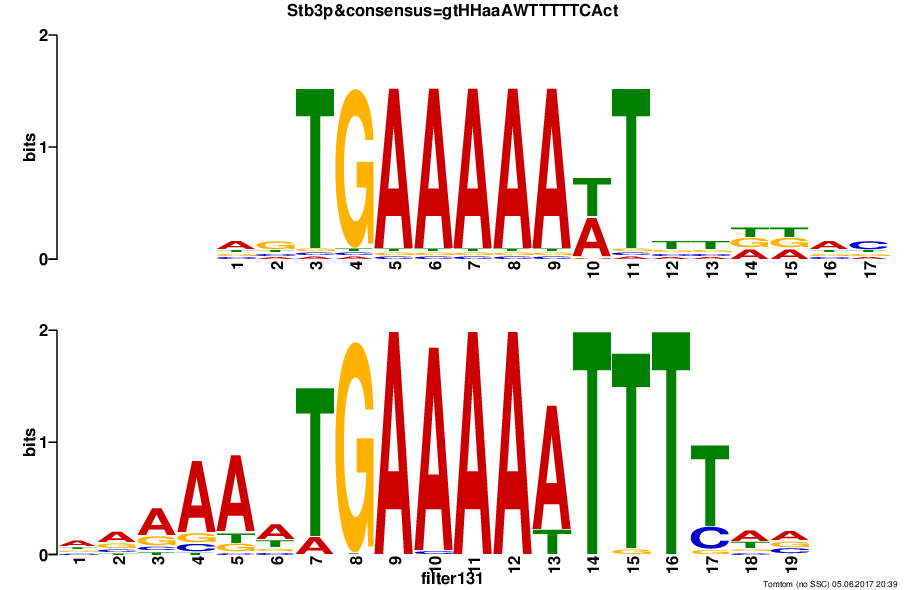
\includegraphics[width=.2\textwidth]{fig/tomtom/stb3p.png}\label{fig:2d}}

\caption{ (a) Predicted vs grounth truth (b-e) examples of recovered motifs}

\end{figure}

\bibliographystyle{unsrt}
\bibliography{references}


\end{document}
